% Chapter 2: Background & State-of-the Art

\chapter{Background \& State of the Art} % Chapter title

\label{chapter:background}
\label{chapter:state-of-the-art}

In this chapter we will introduce and discuss the technical background of this thesis.

We will start by discussing the structure and functionality of multi-core \CPUs and \GPUs.
We will particular focus on \GPUs as their architecture is quite different to traditional \CPUs.
In addition, \GPUs will be the main hardware target of the \SkelCL programming model presented later.
Then we will discuss the most common programming approaches for multi-core \CPUs and \GPUs, with a particular focus on \OpenCL.

We will then introduce structured parallel programming and discuss its foundations in functional programming.
In this approach predefined parallel patterns (\aka, as \emph{algorithmic skeletons}) hiding the complexities of parallelism are used for expressing parallel programs.
This thesis very much builds upon this idea, developing a structured parallel programming model for \GPUs and a novel system compiling pattern-based programs to efficient hardware-specific implementations.
We will finish this chapter by discussing several state-of-the-art implementations of structured parallel programming for cluster systems and multi-core \CPUs.

\section{Modern Parallel Processors}
% structure and functionality of:
As discussed in the introduction virtually all modern processors feature multiple cores to further increase their performance and energy efficiency.
Here we will look at two distinct types of modern parallel processors: multi-core \CPUs and \GPUs.
Multi-core \CPUs are \emph{latency oriented} architectures~\cite{GarlandK10}, \ie, they are optimized to hide memory latencies with large caches and various other advanced architectural features, like out-of-order execution and extensive branch prediction.
\GPUs are \emph{throughput-oriented} architectures~\cite{GarlandK10}, \ie, they are optimized to increase the overall computational throughput of many parallel tasks.

We will discuss both architectures in the following two sections.

\subsection{Multi-Core \CPUs}
% multi-core CPUs
\autoref{fig:multicore} shows an abstract representation of the structural design of a typical multi-core \CPU architecture, like Intel's latest \CPU architecture: Haswell.
\begin{figure}
  \centering
  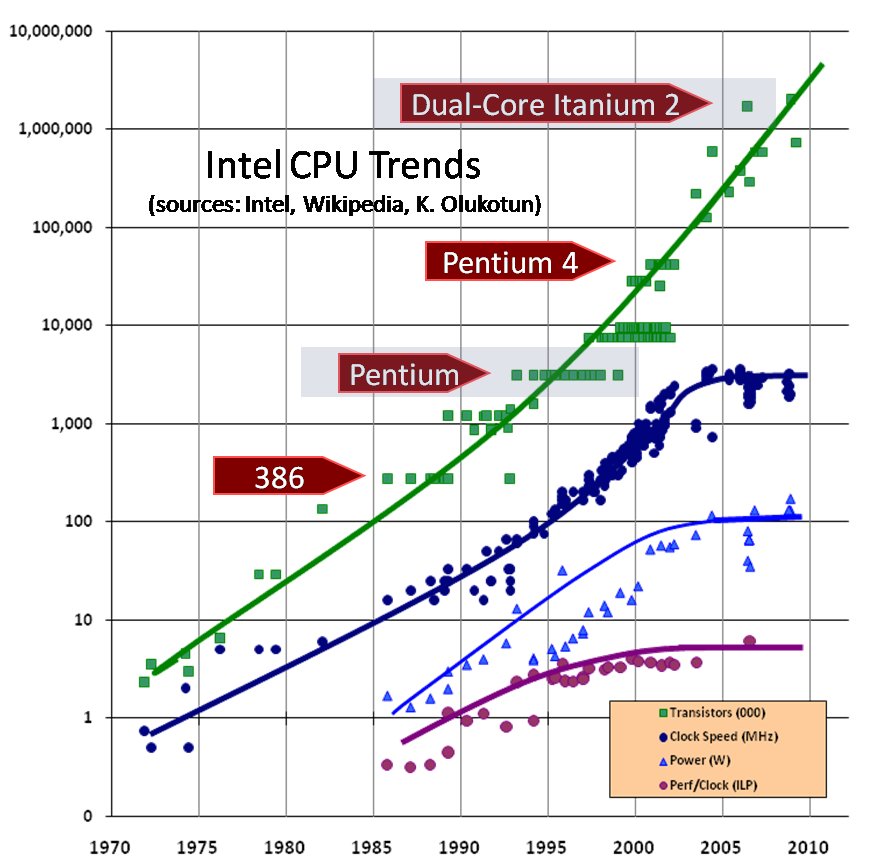
\includegraphics[width=.75\textwidth]{CPU}
  \caption{Multi-core architecture.}
  \label{fig:multicore}
\end{figure}
% describe caches
The \CPU is divided into multiple cores each of which feature two levels of caches.
The smallest but fastest cache is called L1 cache and is typically divided into a distinct cache for instructions and a data cache each of 32 kilobyte for the Haswell architecture.
Each core also features a second level cache (L2 cache) of 256 kilobyte for the Haswell architecture.
The \CPU has a large cache (L3 cache) which is shared by all cores.
This cache is often several megabytes large, for Intel's Haswell architecture the L3 cache is at least 2 and up to 45 megabytes in size.

% describe core: branch prediction, out-of-order execution, SIMD units
Each \CPU core performs computations completely independently of the other cores, but consist itself of multiple execution units which can perform computations in parallel.
This happens transparent to the programmer even when executing a sequential program.
The \CPU core exploits \emph{instruction level parallelism} (ILP) by performing out-of-order execution which reorders instructions prior to execution while still respecting their dependencies.
If two or more instructions have no dependencies they can be executed in parallel.
In the Intel Haswell architecture 4 arithmetic operations and 4 memory operations can be performed in parallel in one clock cycle on every core.
Furthermore, most modern \CPU architectures support SIMD vector extensions like the \emph{Advanced Vector Extensions} (AVX) or the older \emph{Streaming SIMD Extensions} (SSE).
These extensions add additional instructions to the instruction set architecture allowing the compiler to generate code which explicitly groups data into vectors of a small fixed size on which can be operated in parallel.
The current AVX extension allows vectors of up to 256 bits, or the equivalent of grouping and processing 8 single precision floating point numbers in parallel.
Most modern optimizing compilers perform some form of automatic vectorization, but often programmers vectorize programs manually when the compiler fails to generate sufficient optimized code.

% make conclusions: latency oriented => caches important, good performance for single and multiple threads, comparably low core count and hyper threading -> limited thread-level parallelism
The design of multi-core \CPUs is motivated by the overall goal to provide high-performance when executing multi threaded programs and yet still have a high single-core performance when executing sequential programs~\cite{GarlandK10}.
This is why the individual cores are very sophisticated at executing a series of instructions as fast as possible, applying out-of-order execution and featuring other architectural features like a deep pipeline for decoding and executing instructions combined with advanced branch prediction.
Unfortunately, the design of these complex cores make switching between multiple threads running on the same core expensive, as the execution pipeline has to be flushed and the register content for the first thread has to be saved before resuming the execution on the second thread.
To address this issue some multi-core architectures feature \emph{simultaneous multi threading} (SMT), \aka, as \emph{hyper threading}, where a single \CPU core can execute multiple (usually 2 or 4) threads in parallel and switching between the threads is cheap.
His technique is used to mitigate the effect memory latency can have on the execution:
if a thread is waiting for a memory request another thread can continue executing.
The other central component to prevent waiting times for memory requests is the cache hierarchy.
As we will see, multi-core \CPUs feature considerably larger caches than \GPUs.
The caches help to keep the threads running in parallel on the multi-core \CPU busy.

% Possible optimizations
Among the most important optimizations to achieve high performance on these modern multi-core \CPUs are:
exploiting the SIMD extensions and optimizing the cache usage~\cite{IntelCPUOptimizingGuide}.

\subsection{Graphics Processing Units}
  % GPUs
\autoref{fig:gpu} shows an abstract representation of the structural design of a typical \GPU architecture, like Nvidia's latest \GPU architecture for the high-performance computing market: Kepler.
\begin{figure}
  \centering
  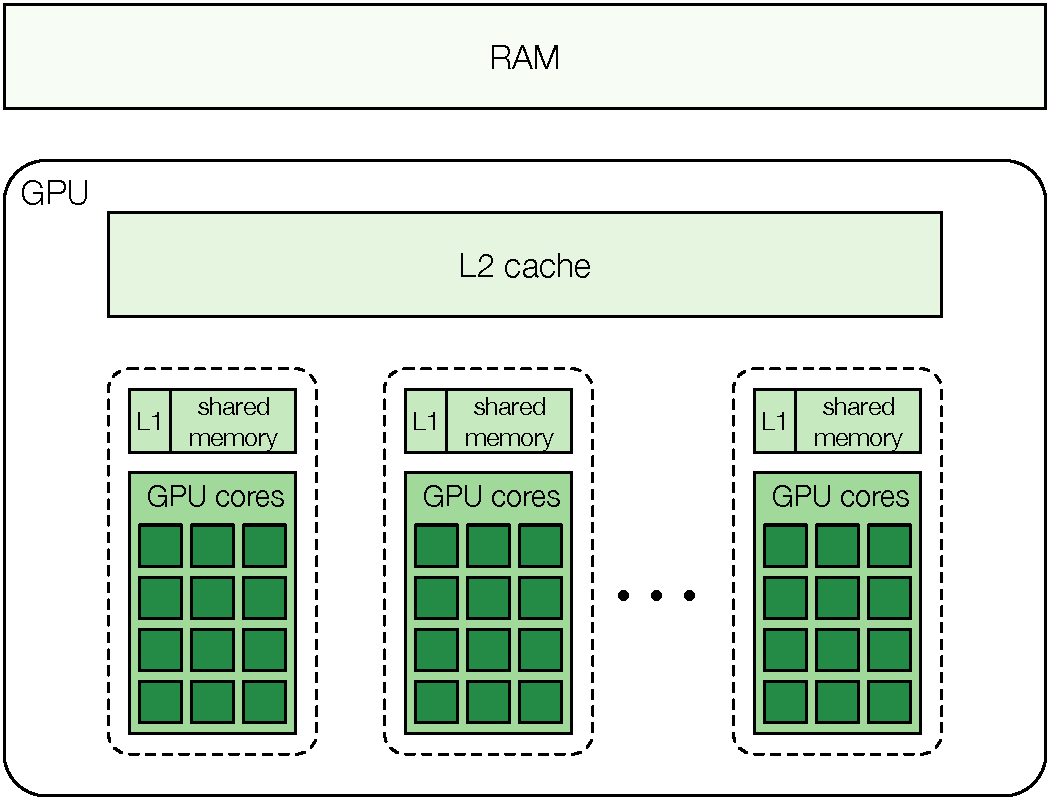
\includegraphics[width=.75\textwidth]{GPU}
  \caption{GPU architecture}
  \label{fig:gpu}
\end{figure}
% describe cores and execution
While the overall design looks fairly similar to the design of the multi-core \CPU the architecture of the \GPU is actually very different in its details.
The lightweight \GPU cores are grouped together into what Nvidia calls a \emph{Streaming Multiprocessor} (SM).
In the Kepler architecture a SM features 192 single-precision cores, 64 double-precision units, 32 special function units, and 32 memory units.
% \autoref{fig:gpuSM} shows the design of a SM in the Kepler architecture.
The 192 single-precision cores are very lightweight compared to the complex \CPU cores we discussed in the previous subsection.
A single \GPU core does not support SIMD vectorization, performs the straightforward in-order execution, and does not perform complex branch prediction.
This design makes the implementation of such a core in hardware very cheap and enables the grouping of hundreds of cores in a single SM.

% describe caches and memory
Modern \GPUs feature two levels of caches:
the first level (L1) is private to each SM and the second level cache (L2) is shared among all SMs.
Compared to the cache sizes of the \CPU the caches on the \GPU are fairly small.
The Kepler architecture features a L1 cache of 48 kilobyte and a L2 cache of 1.5 megabyte.
It is important to notice that these caches are shared by a vast amount of threads being executed on the \GPU:
the 48 kilobyte L1 cache are shared among the up to 2048 threads being executed on the particular SM and the L2 cache is shared among $\approx{}$\!30,\,000 threads.

Besides caches \GPUs also feature a scratchpad memory called \emph{shared memory} in Nvidia's \GPU architectures.
This memory is small (16 or 48 kilobytes) but very fast, comparable to the L1 cache.
Where the L1 cache is automatically managed by a cache controller, the shared memory is explicitly managed by the programmer.

% make conclusions: throughput oriented => cores and threads important, different trade off: poor performance for single thread very good performance for data parallel applications => bad when: a lot of branching, less caches => memory accesses are expensive (coalescing ...)
The design of \GPUs is motivated by the overall goal to deliver maximal throughput even if this requires to sacrifice the performance of single threads~\cite{GarlandK10}.
This is why the \GPU cores are lightweight offering poor sequential performance but thousands of cores combined offering a very high computational throughput.
Memory latencies are mitigated by a high oversubscription of threads:
in the Kepler architecture a SM can manage up to 2048 threads which can be scheduled for execution on the 192 cores.
If a thread is waiting for a memory request another thread continues its execution.
This is the reason why caches are fairly small, as they play a less important role as on in \CPU architectures.

\subsubsection*{\GPU Thread Execution}
The execution of threads on a \GPU is very different compared to the execution on a traditional multi-core \CPU:
multiple threads are grouped by the hardware and executed together.
Such a group of threads is called a \emph{warp} by Nvidia.
In the Kepler architecture 32 threads form a warp and a SM selects 4 warps and for each warp 2 instructions to be executed in parallel on its single-precision cores, double-precision units, special function units, and memory units.

All threads grouped into a warp are forced to perform the same instruction in the same clock cycle.
Is it possible that two or more threads in the same warp have to execute different instructions in the next cycle.
In this case the next instruction from the first threads is chosen and executed by all threads in the warp which have to execute the same instruction.
All threads which do not share the same instructions pause the execution.
In the next cycle the instruction from a thread which had paused before is chosen and executed.
Using this execution strategy threads can be executed together even if they do not have completely identical instruction streams, even though, it is beneficial to group threads which share most instructions, as this reduces the amount of threads pausing their execution.

Programmers are advised to optimize their code, so that threads which will be executed together perform the same instructions.
Threads in the same warp taking different branches in the code can hurt the performance and should, therefore, be avoided if possible.

\subsubsection*{\GPU Memory Accesses}
Accessing the memory is an expensive operation.
The \GPU can optimize accesses when the memory is accesses in certain fixed patterns.
If the threads organized in a warp access a contiguous area of the memory the hardware can \emph{coalesce} the memory access and perform a single memory request instead of issuing individual requests for every thread.
Several other patterns of access exists which are detected by the hardware to coalesce the memory accesses by multiple threads.

This is a major optimization opportunity for many \GPU programs, as the available memory bandwidth can only be utilized properly if memory accesses are coalesced.
Uncoalesced memory accesses offer only a fraction of performance and can severely hurt the performance.


\subsection*{\GPU Shared Memory}
% shared memory

\section{Programming of Multi-Core CPUs and GPUs}
  % programming approaches for multi-core CPUs and GPUs (Threads, OpenMP, CUDA, OpenACC)

\subsection{The OpenCL Programming Model}
    % OpenCL

% structured parallel programming & functional foundations

  % map reduce for clusters

  % TBB for multi-core CPUs


%\from{HIPS begin}
%\section{GPU programming using OpenCL (HIPS)}
%
%The OpenCL standard~\cite{OpenCL} can be used for programming any OpenCL-capable device.
%These devices embrace most modern GPUs and other accelerators, e.\,g., the Cell BE, as well as standard multi-core CPUs.
%
%OpenCL distinguishes between a \emph{host} system, usually containing one or several CPUs, and \emph{devices} that are integrated into the host system.
%An OpenCL device logically consists of one or more \emph{compute units} (CUs) that are divided into one or more \emph{processing elements} (PEs).
%All computation on the device is performed in the PEs.
%OpenCL applications run on the host and call \emph{kernel functions} which are executed simultaneously by multiple PEs on one or more devices.
%A single instance of a kernel function is called a \emph{work-item} and can be identified by its \emph{global ID}.
%Every work-item executes the same code, but the execution can vary per work-item due to branching according to the global ID.
%Work-items are organized in \emph{work-groups}.
%When a kernel function is started, the host code specifies how many work-items are launched and how many work-items form a work-group.
%All work-items in one work-group are executed on the same CU.
%Therefore, the size of a work-group can have a significant effect on the runtime performance.
%
%In OpenCL, host and device have separate memories.
%Thus, functions are provided to transfer data from the host's to the device's memory (\emph{upload}) and back (\emph{download}).
%Memory areas have to be allocated on the device before data can be accessed by it and deallocated thereafter.
%
%For portability across a wide range of devices, kernel functions are compiled at runtime.
%The host program passes the kernel's source code as a plain string to the OpenCL driver to create executable binary code.
%This is different compared to CUDA which provides a special compiler \texttt{nvcc} to compile the device code and the host code.
%
%Creating applications for multi-GPU systems introduces new challenges, like partitioning the application appropriately and, explicitly implementing data transfer between devices~\cite{SchellmannVG08}.
%The host application must coordinate and perform synchronization and data exchange explicitly.
%The source code for performing such exchanges further increases the amount of boilerplate code.
%
%In the following, we describe how our SkelCL library addresses these problems of GPGPU programming.
%\from{HIPS end}
%
%
%\from{HiStencils begin}
%\section{Stencils Using OpenCL (HiStencils)}
%\label{sec:background}
%
%A \emph{stencil computation} is a computation pattern on a multi-dimensional grid, where each point of the grid is updated (often iteratively) as a function of its neighboring points.
%Each point of the grid stores a set of application-dependent values.
%The computation performed to update the values of each point is called the \emph{stencil operation}.
%A stencil operation updates the value of a point depending on the values of the neighboring points.
%The points taken into account for a stencil operation are defined by the \emph{stencil shape}.
%
%Let us consider how stencil computations are implemented on manycore systems with GPUs using the state-of-the-art OpenCL standard.
%Listing~\ref{lst:sobel_opencl} presents the structure of an OpenCL implementation of the Sobel operator on one GPU, a typical stencil computation used in image processing for detecting edges in images.
%Lines 9--13 show how the direct neighboring elements, e.g., the \emph{upper left} (\texttt{ul}) neighbor, are accessed and passed to a function performing the Sobel operation in line 16.
%Many low-level details have to be considered for a correct implementation, like raw pointer handling, including index computations (e.g., line 10), and explicit out-of-bound  accesses handling (e.g., line 9).
%
%\begin{lstlisting}[%
%caption={Structure of the OpenCL implementation of Sobel edge detection},%
%float=tbp,%
%label={lst:sobel_opencl}]
%kernel
%  void sobel(global const char* in_img,
%             global char* out_img,
%             int w, int h) {
%  int i = get_global_id(0);
%  int j = get_global_id(1);
%
%  if (i < w && j < h) {
%    char ul = (j-1 > 0 && i-1 > 0)
%        ? in_img[((j-1)*w)+(i-1)] : 0;
%    ...
%    char lr = (j+1 < h && i+1 < w)
%        ? in_img[((j+1)*w)+(i+1)] : 0;
%
%    out_img[j*w+i] =
%        computeSobel(ul, ..., lr);
%  }
%}
%\end{lstlisting}
%
%The OpenCL version is obviously correct, but not efficient:
%the fast local GPU memory is not used and the control flow diverges heavily between different work items, which is disadvantageous on current GPU architectures.
%However, the corresponding optimizations require a deep knowledge of the GPU's architecture and must be programmed and tuned manually and are, therefore, a complicated task for application developers.
%If the program is to be used on a multi-GPU system then the application developer has to additionally implement and optimize the explicit data distribution across GPUs and the communication between them.
%\from{HiStencils end}
%
%\from{PACT begin}
%\section{OpenCL (PACT)}
%\paragraph{OpenCL Execution Model}
%OpenCL can be used to program manycore CPUs and GPUs.
%Both are typically represented in the system as an accelerator.
%Programming these devices consists of writing a compute \emph{kernel} in OpenCL C that executes on the device and writing the host code that orchestrates data movement, allocates memory and manages the execution on the device.
%
%\paragraph{Thread Organization and Synchronization}
%Most GPUs are organized as multicore processors with each core executing multiple threads concurrently.
%OpenCL represents this with the concept of \emph{workgroups} that contain \emph{local threads}.
%Threads within a core are typically grouped in \emph{warps} (using Nvidia terminology) where each thread executes in a lock-step synchronized manner.
%Only one warp is active at a time and execution switches to a different warp when the pipeline stalls to hide memory latency.
%OpenCL allows to synchronize threads at the kernel level on the host or at the workgroup level using a barrier function synchronizing the local threads.
%Threads within a warp are implicitly synchronized on GPUs.
%
%
%\paragraph{Vector Units}
%Most modern CPUs and devices such as AMD GPUs integrates vector units that can process more than on data element at a time.
%The OpenCL programming model exposes this with special data types such as \texttt{int4} where any operations on this type will be executed in the vector units.
%In the absence of vector units in the hardware, the OpenCL compiler scalarizes the code automatically.
%
%\paragraph{Memory Coalescing}
%On GPUs, requests to the main device memory are usually performed at the granularity of a cache line, which is typically 64 bytes.
%Therefore, due to the organization of the threads in warps, it is important to ensure that consecutive threads access consecutive memory elements to maximize memory bandwidth.
%
%\paragraph{Local Memory}
%Most GPUs have a per-core cache and a local memory shared among all local threads.
%OpenCL defines a global and local address space.
%On GPUs, local memory has a high bandwidth and low latency and is used to store frequently accessed data.
%On CPUs, local memory is usually simply mapped to a region of global memory.
%\from{PACT end}

% include related work
%\section{Related work}

\from{HIPS begin}
\subsection{HIPS}
% ------------------------------------------------------------------------------

There are a number of other projects aiming at high-level GPU programming.

\emph{SkePU}~\cite{EnmyrenKe10} uses container classes and algorithmic skeletons to ease multi-GPU computing.
Although SkePU and SkelCL have been developed independently, both projects share some concepts:
SkePU provides a vector class similar to SkelCL's \texttt{Vector} class, but unlike SkelCL it does not support different kinds of data distribution on multi-GPU systems.
SkePU and SkelCL both provide a map and a reduce skeleton.
However, SkelCL additionally provides the \texttt{Zip} and \texttt{Scan} skeleton, while SkePU supports two additional variants of the map skeleton.
Unlike SkelCL, which allows for an arbitrary number of arguments, in SkePU the user-defined functions are restricted to a fixed skeleton-specific number of arguments.
Currently, SkePU is the only project other than SkelCL that supports data-parallel computations on multi-GPU systems.
SkelCL provides a more flexible memory management than SkePU, as data transfers can be expressed by changing data distribution settings.
Only this flexibility provides the best performance for our second case study (Section~\ref{sec:list-mode_OSEM}) and similar applications.
Both projects differ significantly in the way how functions are passed to skeletons.
While functions are defined as plain strings in SkelCL, SkePU uses a macro language, which brings some serious drawbacks.
For example, it is not possible to call mathematical functions like sin or cos inside a function generated by a SkelPU macro,
because these functions are either named differently in all three target programming models or might even be missing entirely.
The same holds for functions and keywords related to performance tuning, e.\,g., the use of local memory.
SkelCL does not suffer from these drawbacks because it relies on OpenCL and thus can be executed on a variety of devices.

\emph{CUDPP}~\cite{SenguptaHZO07} is a C++ library based on CUDA.
It provides data-parallel algorithm primitives similar to skeletons.
These primitives can be configured using only a predefined set of operations, whereas
skeletons in SkelCL are true higher-order functions, which accept any user-defined function.
CUDPP does not simplify data management, because data still has to be exchanged between CPU and GPU explicitly.
There is also no support for multi-GPU applications.

\emph{Thrust}~\cite{BellHo2011} is an open-source library by NVIDIA.
It provides two vector types similar to the vector type of the C++ Standard Template Library.
While these types refer to vectors stored in CPU or GPU memory, respectively, SkelCL's vector data type provides a unified abstraction for CPU and GPU memory.
Thrust also contains data-parallel implementations of higher-order functions, similiar to SkelCL's skeletons.
SkelCL adopts several of Thrust's ideas, but it is not limited to CUDA-capable devices and supports multiple GPUs.

Unlike SkelCL, \emph{PGI Acccelerator}~\cite{PGI-10} and \emph{HMPP}~\cite{HMPP-09} are compiler-based approaches to GPU programming, similar to the popular OpenMP~\cite{OpenMP-08}.
The programmer uses compiler directives to mark regions of code to be executed on a GPU.
A compiler generates executable code for the GPU, based on the used directives.
Although source code for low-level details like memory allocation or data exchange is generated by the compiler, these operations still have to be specified explicitly by the programmer using suitable compiler directives.
We consider these approaches low-level, as they do not perform data transfer automatically to shield the programmer from low-level details.
\from{HIPS end}

\from{ASHES begin}
\subsection{ASHES}
SkelCL is a runtime, library-based approach for GPU programming, unlike compiler-based approaches, e.\,g., \emph{HMPP}~\cite{HMPP-07} and the \emph{PGI Accelerator compilers}~\cite{PGI-10}.
It offers the user a consistent high-level API while still allowing the programmer to use all features of the underlying OpenCL standard.

There are other library-based approaches for high-level GPU programming.

\emph{SkePU}~\cite{EnmyrenKe10} is a skeleton-based framework for multi-core CPUs and multi-GPU systems.
An architecture-independent macro language is used which, however, makes architecture-specific optimizations impossible, like the use of local memory in OpenCL.
SkelCL avoids this drawback by building on top of OpenCL.
SkePU provides memory abstractions similar to SkelCL, but does not support different data distributions on multi-GPU systems as in SkelCL:
vectors are always distributed to all available devices, with no possibility of data exchanges between devices.
Therefore, our list-mode OSEM application which heavily relies on multiple data exchanges between devices cannot be implemented efficiently using SkePU.

\emph{Thrust}~\cite{BellHo2011} provides an interface similar to the C++ Standard Template Library (STL).
For data management, two distinct dynamic containers, a \texttt{host\_vector} and a \texttt{device\_vector}, can be used like STL vectors for managing host and device memory respectively.
% Data is copied to a device by assigning a \texttt{host\_vector} to a \texttt{device\_vector}.
In addition, Thrust offers common parallel algorithms, including searching, sorting, reductions, and transformations.
Thrust is based on CUDA, therefore, restricting the user to NVIDIA GPUs.

\emph{GPUSs}~\cite{AyBILMQ-09} is an implementation of the Star Superscalar model for multi-GPU systems.
While SkelCL is focused on data parallelism, GPUSs provides simple task parallelism;
annotations are used for data transfers between host and GPU.
SkelCL offers a higher level of memory abstraction: communication is specified implicitly by a distribution scheme instead of individual data transfers.

Rabhi and Gorlatch~\cite{RaG-03} present different approaches of skeletal programming for parallel as well as distributed systems.
Gonz\'{a}lez-V\'{e}lez and Leyton~\cite{GoL-10} provide an overview of available skeleton frameworks.
\from{ASHES end}

\from{ICCS begin}
\subsection{ICCS}
A considerable amount of work exists in the filed of algorithmic skeletons;
for an overview we refer to~\cite{gc11}.
There are several related approaches to raise the level of program abstraction in GPU programming.
While SkelCL can be used for programming multiple OpenCL capable GPUs, the CUDA-based \emph{Thrust}~\cite{BellHo2011} library simplifies programming only for a single NVIDIA GPU.
As SkelCL, \emph{SkePU}~\cite{EnK-10} is a skeleton library targeting multi-GPU systems.
In contrast to our work which is based entirely on the portable OpenCL, SkePU is implemented with multiple back-ends which restrict the application developer to the back-ends' smallest common set of functions and, thus, prevents the user from applying optimizations, like using the fast local GPU memory.
\from{ICCS end}

\from{HLPP begin}
\subsection{HLPP}
Considerable theoretical as well as practical research has been conducted in the field of algorithmic skeletons since its introduction in the late 1980s.
Due to lack of space, we refer to~\cite{GoC-11} for an overview of skeletal programming and~\cite{gl10} for a recent survey of skeleton libraries for clusters and multi-core CPUs.
Our contribution to skeletal programming is the introduction and efficient implementation of a new algorithmic skeleton for performing allpairs computations.
As other skeletons, the allpairs skeleton can be used as a basic building block by application developers who do not have to be experts in GPU computing or parallel programming in general.

In previous work, efficient parallel implementations of allpairs computations on modern parallel processors were studied (e.\,g., multi-core CPUs~\cite{AroraShVu2009}, the Cell processor~\cite{WirawanSK09}, and GPUs~\cite{ChangDeQuRo2009}) in the context of specific applications.
In contrast to~\cite{SarjeAl2013}, which presents an efficient implementation scheme of allpairs computations for GPUs, we abstract the computation as an algorithmic skeleton and offer its efficient implementation to application developers as part of the SkelCL skeleton library.

The evaluation of the programming effort shows that the allpairs skeleton allows to express many applications considerably shorter and at a higher level of abstraction, as compared to using OpenCL or library implementations like BLAS.
The performance comparison shows that by making information about the memory access pattern available to the implementation, we can considerably improve the performance by efficiently using the fast GPU local memory.

Several current approaches address simplifying GPU programming.
As SkelCL, also SkePU~\cite{EnmyrenKe10} and Muesli~\cite{ErK-12} are skeleton libraries targeting multi-GPU systems.
In contrast to our work, which is based entirely on the portable OpenCL, Muesli is implemented using NVIDIA's CUDA and SkePU is implemented with multiple back-ends which restrict the application developer to the back-ends' smallest common set of functions.
While SkelCL can be used for programming multiple OpenCL-capable GPUs, the CUDA-based Thrust~\cite{BellHo2011} library simplifies programming only for a single NVIDIA GPU.
\from{HLPP end}

\from{PaCT begin}
\subsection{PaCT}
There are a number of other projects aiming at high-level GPU programming.

\emph{SkePU}~\cite{EnmyrenKe10} provides a vector class similar to our \texttt{Vector} class, but unlike SkelCL it does not support different kinds of data distribution on multi-GPU systems.
SkelCL provides a more flexible memory management than SkePU, as data transfers can be expressed by changing data distribution settings.
Both approaches differ significantly in the way how functions are passed to skeletons.
While functions are defined as plain strings in SkelCL, SkePU uses a macro language, which brings some serious drawbacks.
For example, it is not possible to call mathematical functions like sin or cos inside a function generated by a SkelPU macro,
because these functions are either named differently in all of their three target programming models (CUDA, OpenCL, OpenMP) or might even be missing entirely.
The same holds for functions and keywords related to performance tuning, e.\,g., the use of local memory.
SkelCL does not suffer from these drawbacks because it relies on OpenCL and thus can be executed on a variety of GPUs and other accelerators.

\emph{CUDPP}~\cite{SenguptaHZO07} provides data-parallel algorithm primitives similar to skeletons.
These primitives can be configured using only a predefined set of operations, whereas
skeletons in SkelCL are true higher-order functions which accept any user-defined function.
CUDPP does not simplify data management, because data still has to be exchanged between CPU and GPU explicitly.
There is also no support for multi-GPU applications.

\emph{Thrust}~\cite{BellHo2011} provides two vector types similar to the vector type of the C++ Standard Template Library.
While these types refer to vectors stored in CPU or GPU memory, respectively, SkelCL's vector data type provides a unified abstraction for CPU and GPU memory.
Thrust also contains data-parallel implementations of higher-order functions, similiar to SkelCL's skeletons.
SkelCL adopts several of Thrust's ideas, but it is not limited to CUDA-capable GPUs and supports multiple GPUs.

Unlike SkelCL, \emph{OpenACC}~\cite{OpenACC}, \emph{PGI Acccelerator}~\cite{PGI-10}, and \emph{HMPP}~\cite{HMPP-09} are compiler-based approaches to GPU programming, similar to the popular OpenMP~\cite{OpenMP-08}.
The programmer uses compiler directives to mark regions of code to be executed on a GPU.
A compiler generates executable code for the GPU, based on the used directives.
Although source code for low-level details like memory allocation or data exchange is generated by the compiler, these operations still have to be specified explicitly by the programmer using suitable compiler directives.
We consider these approaches low-level, as they do not perform data transfer automatically to shield the programmer from low-level details and parallelism is still expressed explicitly.
\from{PaCT end}

\from{HiStencils begin}
\subsection{HiStencils}
Several approaches aiming at simplifying GPU programming exist.
\emph{SkePU}~\cite{EnmyrenKe10} provides a vector class similar to our \texttt{Vector} class, but unlike SkelCL it does not support different kinds of data distribution on multi-GPU systems.
SkelCL provides a more flexible memory management than SkePU, as data transfers can be expressed by changing data distribution settings.
\emph{Thrust}~\cite{BellHo2011} provides two vector types similar to the vector type of the C++ Standard Template Library.
While these types refer to vectors stored in CPU or GPU memory, respectively, SkelCL's vector data type provides a unified abstraction for CPU and GPU memory.
Thrust also contains data-parallel implementations of higher-order functions, similiar to SkelCL's skeletons.
SkelCL adopts several of Thrust's ideas, but it is not limited to CUDA-capable GPUs and supports multiple GPUs.
Both SkePU and Thrust provide no explicit support for stencil computations.

Several projects focus on stencil computations on GPUs.
PATUS~\cite{PATUS} is a code generation and tuning framework for stencil computations.
It can generate optimized code for multicore processors and a single GPU.
PARTANS~\cite{PARTANS} is a code generation and autotuning framework for stencil computations on multiple GPUs. 
It automatically distributes and optimizes stencil computations on multiple GPUs, by searching for optimal parameters for a given hardware architecture.
These specialized domain-specific approaches can only be applied to stencil computations, whereas SkelCL is a general-purpose approach.
\from{HiStencils end}


\from{PACT begin}
\subsection{PACT}

\paragraph{Algorithmic Patterns}
Algorithmic patterns or skeletons~\cite{cole88skeleton} have been around for more than two decades.
The Map-Reduce~\cite{dean08mapreduce} framework from Google for instance allows programmers to express computation using two operators; map and reduce.
Since the original framework was developed, many researchers have looked at the problem of optimizing these operations for different type of hardware.
Paraprox~\cite{Samadi14Paraprox} for instance uses automatic detection of algorithmic patterns to apply optimization at the expense of accuracy.
Compared to our approach, most prior works rely on hardware-specific implementations to achieve high performance.
Conversely, we automatically generate implementations using our fine-grain hardware patterns combined with our rule rewriting system.

\paragraph{Functional Approaches for GPU Code generation}
Accelerate is a functional domain specific language built within Haskell to support GPU acceleration~\cite{chakravarty11accelerating,mcdonell13optimising}.
Recently, Nvidia has released technical reports on NOVA~\cite{collins13nova}, a new functional language target at code generation for GPUs, and Copperhead~\cite{catanzaro11copperhead}, a data parallel language embedded in Python.
Nova shares many concepts from Accelerate and Copperhead and offers familiar data parallel patterns.
HiDP~\cite{zhang13hidp} is a hierarchical data parallel language which maps computations to the OpenCL programming model similar to our approach.
All these projects rely on analysis of user code or hand-tuned versions of high-level algorithmic patterns.
In contrast, our approach uses rewrite rules and low-level hardware patterns to produce high-performance code in a portable way.

\paragraph{Rewrite-rules for Optimizations}
Rewrite rules have been used very early as a way to automate the optimization process of functional programs~\cite{jones01playing}.
Similar to us, Spiral~\cite{pueschel05spiral,Spampinato13LGen} also uses rewrite rules to optimize signal processing programs and was more recently adapted to other applications such as linear algebra.
Chellappa et al. show how Spiral can be used to automatically parallelize code for the IBM Cell BE processor~\cite{Chellappa09computer}.
In contrast our rules and hardware patterns are expressed at a much finer level, allowing for highly specialized and optimized code generation.

\paragraph{High-level Code Generation for GPUs} 
A large body of work has explored how to automatically generate high performance code for GPUs.
Dataflow programming models such as IBM's LiquidMetal~\cite{dubach12compiling} or StreamIt~\cite{thies02streamit} have been used to automatically produce GPU code with OpenCL or CUDA~\cite{hormati11sponge,huynh12scalable,udupa09software}.
Directive based approach have also been used such as OpenMP to CUDA~\cite{lee09openmp}, OpenACC to OpenCL~\cite{reyes12openaccgpu}, or hiCUDA~\cite{han11hicuda} which translates sequential C code to CUDA.
Other works include the automatic mapping of data-parallel programs to the IBM Cell processor~\cite{Wang09automatic}.
Delite~\cite{brown11heterogeneous,chafi11domain}, a system that enables the creation of domain-specific languages, can also target mutlicore CPUs or GPUS.
Unfortunately, all these approaches do not provide full performance portability since the mapping of the application assumes a fixed platform and the optimizations and implementations are targeted at a specific device.
X10~\cite{charles05x10}, a language for high performance computing, can also be used to program GPUs~\cite{cunningham11gpu}.
However, the programming style remains low-level since the programmer has to express in X10 the same low-level operations found in CUDA or OpenCL.

Recently, researchers have looked at generating efficient GPU code for loops using the polyhedral framework~\cite{verdoolaege13polyhedral}.
This framework enables the exploration of various optimizations such as use of local memory or vectorization.
Finally, Petabricks~\cite{ansel09petabricks} takes a different approach by letting the programmer specify different algorithms implementations.
The compiler and runtime then choose the most suitable one based on an adaptive mechanism and can produce OpenCL code~\cite{phothilimthana13portable}.
Compared to our work, they generate optimized code by relying on static analysis.
Our code generator does not make any decisions nor perform any analysis since the optimization process happens at a higher level within our rewrite rules.
\from{PACT end}


